% Intended LaTeX compiler: pdflatex
\documentclass[10pt,a4paper,UTF8]{article}
\usepackage{zclorg}
\usepackage{tikztheorem}
\author{zcl.space}
\date{}
\title{使用matlab的surface和contour画图}
\hypersetup{
 pdfauthor={zcl.space},
 pdftitle={使用matlab的surface和contour画图},
 pdfkeywords={matlab surface contour},
 pdfsubject={},
 pdfcreator={Emacs 25.2.1 (Org mode 9.0.9)},
 pdflang={English}}
\begin{document}

\maketitle
\tableofcontents
\titlepic{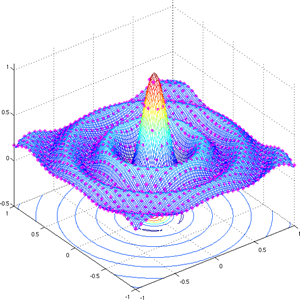
\includegraphics[scale=0.25]{../../img/sinc.PNG}}

\section{简介}
\label{sec:org2200315}


matlab提供了两个酷炫的函数\href{https://www.mathworks.com/help/matlab/ref/surface.html?searchHighlight=surface\&s\_tid=doc\_srchtitle}{surface} 和\href{https://www.mathworks.com/help/matlab/ref/contour.html?searchHighlight=contour\&s\_tid=doc\_srchtitle}{contour} 用来画多维函数的图形。通过这两个函数我们可以对多维函数进行更直观的观察。

本文以函数:
\begin{equation}
\label{eq:1}
z = x\exp(-x^{2} + y^{2})
\end{equation}
为例,介绍 surface和contour的实用方法。

\section{surface}
\label{sec:org1dc47c9}


看代码:
\lstset{language=matlab,label= ,caption= ,captionpos=b,firstnumber=1,numbers=left}
\begin{lstlisting}
[X,Y] = meshgrid(-2:0.2:2,-2:0.2:2);
Z = X.*exp(-X.^2 - Y.^2);
figure
surface(X,Y,Z)
view(3)
\end{lstlisting}

结果如图:
\begin{figure}[htbp]
\centering
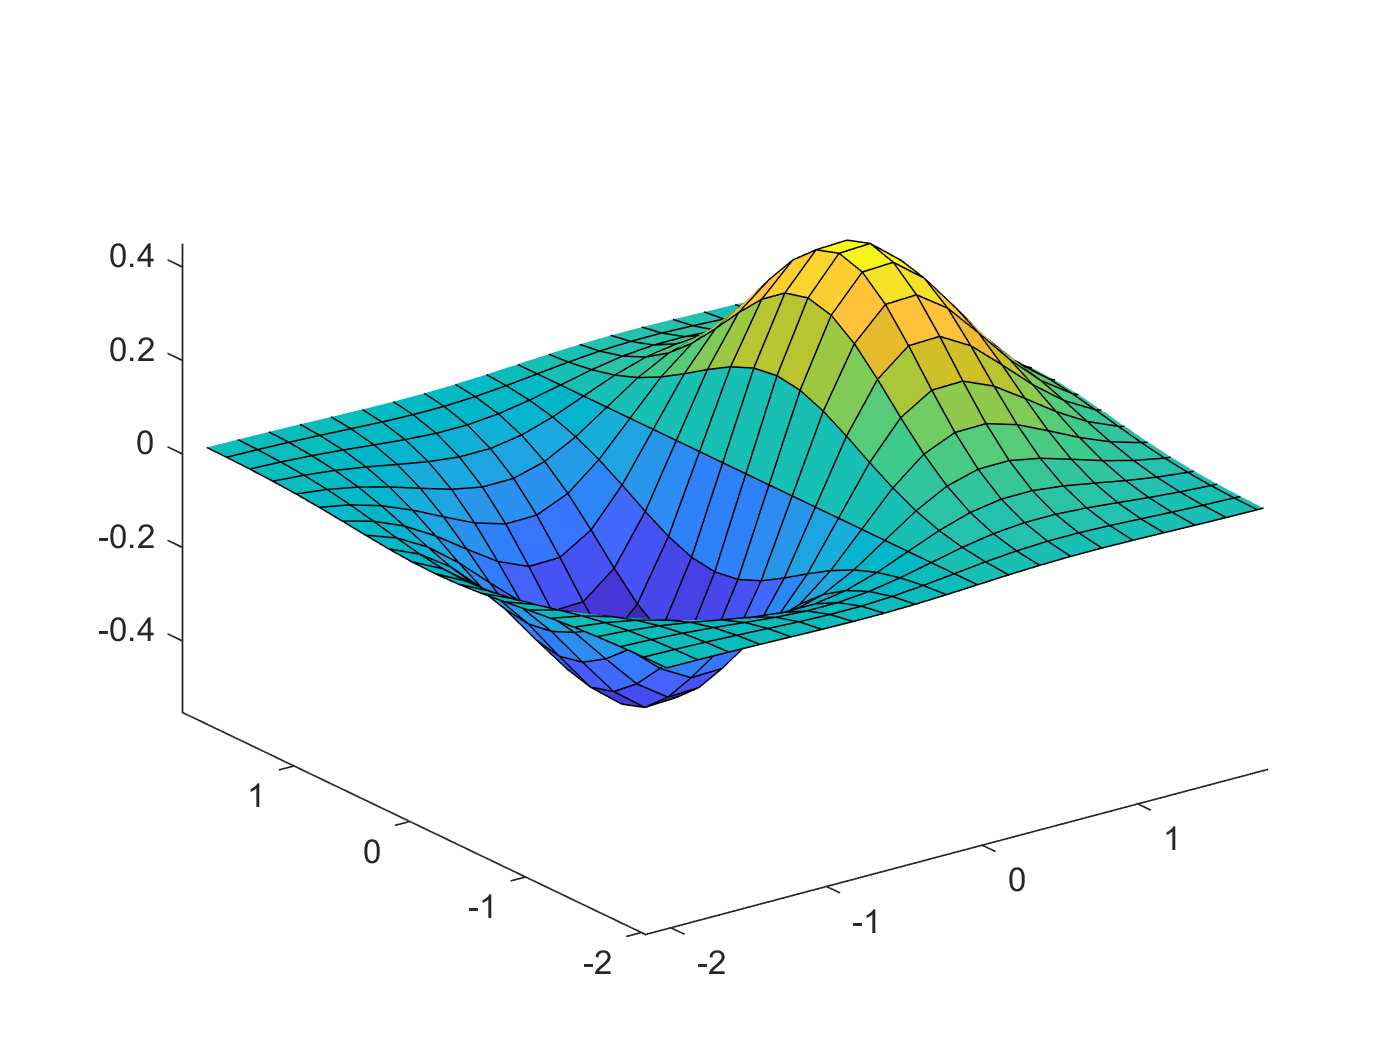
\includegraphics[width=0.6\textwidth]{../../img/communication_matlab/20170708surface.png}
\caption{\label{fig:org2498ddf}
surface示例}
\end{figure}

注意在画图的时候,最后一句 \texttt{view(3)} 是必须的。不然matlab会默认使用 \texttt{view(2)} ,看到的会是二维的平面截图。

\section{contour}
\label{sec:orga28b7ee}


contour 的功能是画一个多维函数的等高线。

看代码:
\lstset{language=matlab,label= ,caption= ,captionpos=b,firstnumber=1,numbers=left}
\begin{lstlisting}
x = -2:0.2:2;
y = -2:0.2:3;
[X,Y] = meshgrid(x,y);
Z = X.*exp(-X.^2-Y.^2);

figure
contour(X,Y,Z,'ShowText','on')
\end{lstlisting}

结果如图:
\begin{figure}[htbp]
\centering
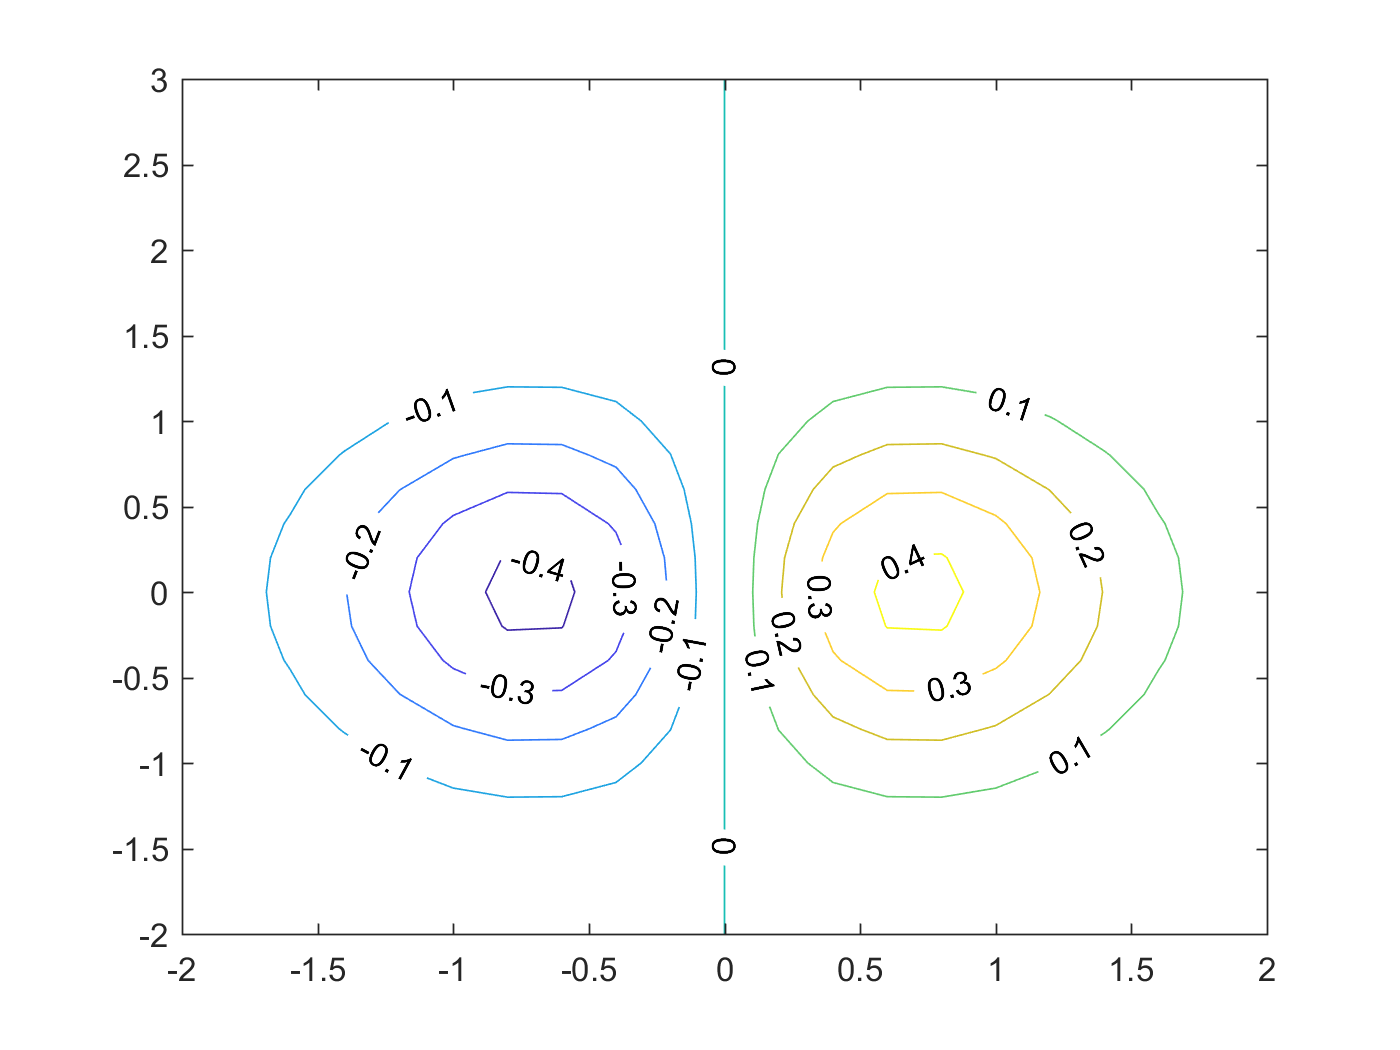
\includegraphics[width=0.6\textwidth]{../../img/communication_matlab/20170708contour.png}
\caption{\label{fig:org2b7b2e3}
contour示例}
\end{figure}

matlab的帮助手册中有关于contour的更详细的说明,包括一些画图的技巧,等高线的间隔,高亮某条等高线等等。

\section{gradient}
\label{sec:org4bde28f}


在contour的基础上,我们看看\(xe^{-x^{2} - y^{2}}\)的梯度示意图。
\lstset{language=matlab,label= ,caption= ,captionpos=b,firstnumber=1,numbers=left}
\begin{lstlisting}
x = -2:0.2:2;
y = x';
z = x .* exp(-x.^2 - y.^2);
[px,py] = gradient(z);
figure
contour(x,y,z)
hold on
quiver(x,y,px,py)
hold off
\end{lstlisting}

结果如下:
\begin{figure}[htbp]
\centering
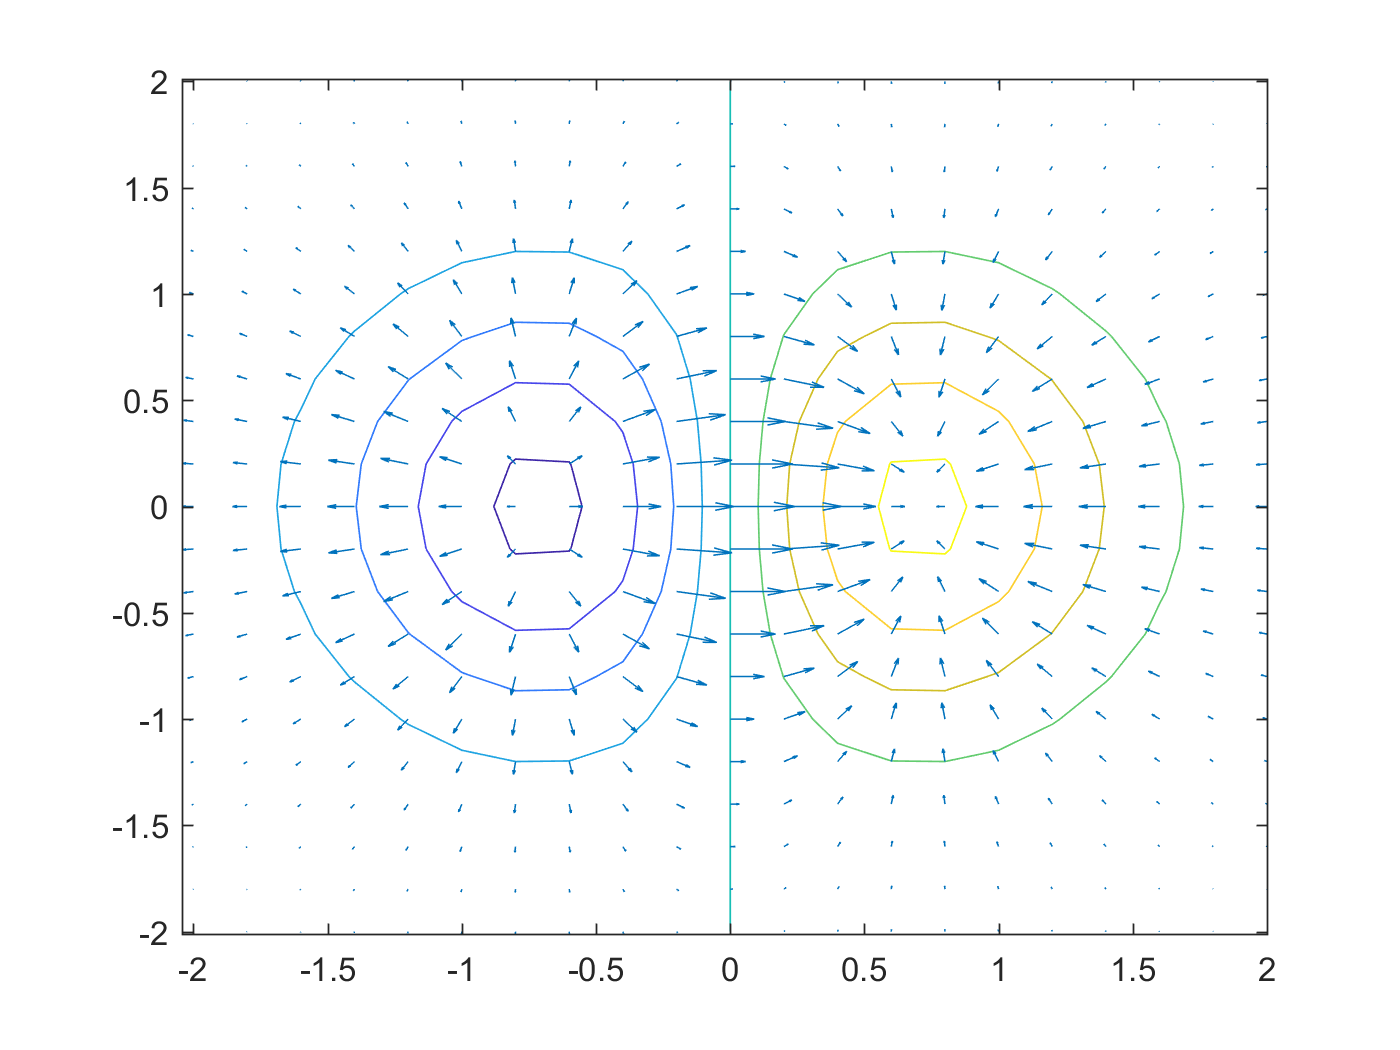
\includegraphics[width=0.6\textwidth]{../../img/communication_matlab/20170708gradient.png}
\caption{\label{fig:org11a1b3d}
\(xe^{-x^{2} - y^{2}}\)的梯度示意图}
\end{figure}

图\ref{fig:org11a1b3d}中的箭头所指是图\ref{fig:org2498ddf}中从蓝色到橙色,即箭头部分永远指向更高的位置。
\end{document}
